\section{Matchings und Maximum Independent Set}

\texttt{MAXIMUM INDEPENDENT SET}: Für $G = (V, E)$, finde eine \textbf{größte unabhängige Menge}.
Also Knotenmenge $I\subseteq V$ mit $|I|$ maximal, sodass jede Kante in $E$ höchstens einen Endpunkt in $I$ hat.\\

\textbf{Approximationsalgorithmus für \texttt{MAXIMUM INDEPENDENT SET}}:
\begin{enumerate}
	\item Zerkleinere den Graphen mit Planar Separator, bis Komponenten nur noch $\mathcal{O}(\log\log n)$ Knoten haben
	\item Löse Komponenten mit Brute-Force in $\mathcal{O}(2^{\log\log n})= \mathcal{O}(\log n)$ Zeit pro Komponente $\rightarrow$ $\mathcal{O}(n\log n)$ Gesamtlaufzeit
	\item Zusammenfügen ist disjunkte Vereinigung der Teillösungen (Kein Problem an Schnittpunkten, da Separator dazwischen)
\end{enumerate}
\medskip
\textbf{Güte der Approximation}:

\begin{itemize}
	\item \textbf{Satz}: Wiederholtes Anwenden des planar Separators gibt Komponenten der Größe $\mathcal{O}(r)$ bei Separator-Gesamtgröße $\mathcal{O}(n/\sqrt{r})$
	
	\textit{ohne Beweis.}
	
	\item Mit obigem Satz folgt Separator-Gesamtgröße $|S|\leq\mathcal{O}(n/\sqrt{\log\log n})$
	\item Für optimale Lösung $OPT(G)$ gilt $OPT(G)\geq n/4$ nach Vier-Farben-Satz
	\item Damit folgt:
	$$
	\begin{aligned}
		& OPT(G)-A(G) \leq|S| \leq \mathcal{O}\left(\frac{n}{\sqrt{\log \log n}}\right) \\
		\Rightarrow A(G) & \geq OPT(G)-\mathcal{O}\left(\frac{n}{\sqrt{\log \log n}}\right) \\
		& \geq OPT(G)-\mathcal{O}\left(\frac{OPT(G)}{\sqrt{\log \log n}}\right) \\
		& =OPT(G) \cdot\left(1-\mathcal{O}\left(\frac{1}{\sqrt{\log \log n}}\right)\right)
	\end{aligned}
	$$
	wobei $OPT(G)-A(G) \leq|S|$ gilt, da $A$ für die Separatoren keine Lösungen berechnet und somit die Abweichung von der optimalen Lösung max. so groß ist wie die Kardinalität von $S$.
\end{itemize}
\bigskip
\textbf{Definition}:
\begin{itemize}
	\item Kantenmenge $M$ ist ein \textbf{Matching} wenn jeder Knoten zu höchstens einer Kante in $M$ inzident ist.
	\item Wenn ein Knoten $v$ zu einer Kante in $M$ inzident ist, heißt $v$ \textbf{gematcht}, ansonsten \textbf{ungematcht}.
	\begin{center}
		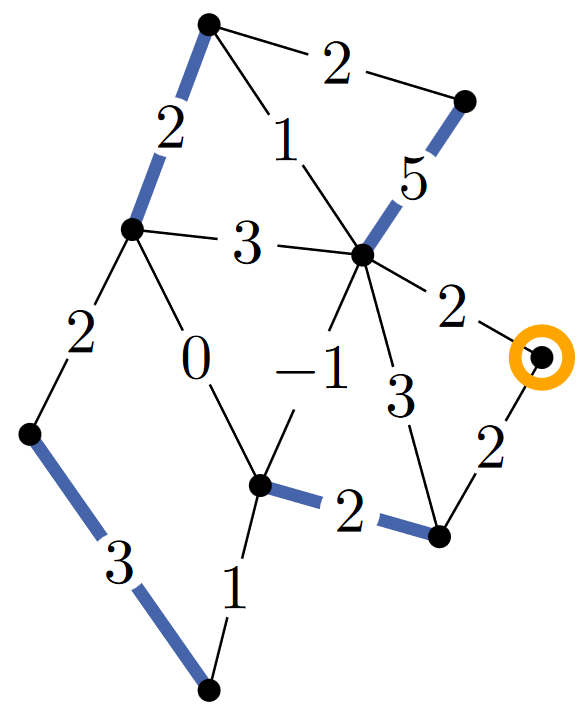
\includegraphics[width=0.2\textwidth]{images/matching.png}
	\end{center}
\end{itemize}
\bigskip
\texttt{GEWICHTSMAXIMALES MATCHING}: 
\begin{itemize}
	\item \textbf{Gegeben}: Graph $G=(V,E)$ und Gewichtsfunktion $w\colon E\rightarrow\R$
	\item \textbf{Gesucht}: Matching $M\subseteq E$ mit $w(M)=\sum\limits_{e\in M} w(e)$ maximal
\end{itemize}
\bigskip
\textbf{Definition}: Sei $M\subseteq E$ Matching in $(G = (V, E), w)$. Ein $M$-alternierender Weg ist ein einfacher Pfad oder Kreis $P$ in $G$, sodass
\begin{itemize}
	\item sich Kanten von $M$ und $E- M$ auf $P$ abwechseln
	\item wenn $P$ ein Pfad mit Endpunkt $v$ und Kante $e$ an $v$ in $P$ ist, dann ist $e\in M$ oder $v$ ungematcht (verhindert, dass der Pfad verlängert werden kann)
	\begin{center}
		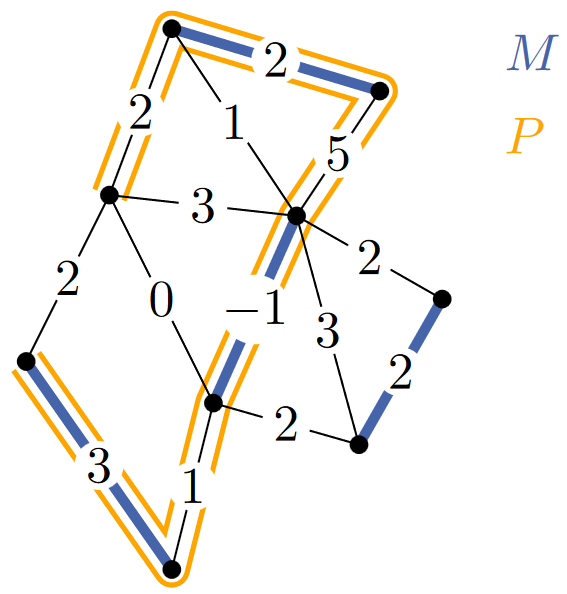
\includegraphics[width=0.2\textwidth]{images/alternating-path.png}
	\end{center}
\end{itemize}
Für Matching $M$ und alternierenden Weg $P$ ist auch $M\Delta P\coloneqq (M- P)\cup(P- M)$ (\textbf{symm. Differenz}) ein Matching.

Dabei gilt $w(M\Delta P)-w(M)=w(P- M)-w(P\cap M)$, denn sowohl neues Matching als auch altes Matching enthalten die Kanten, die nicht auf dem Pfad liegen. Dann ist die Differenz zwischen neuem und alten Matching nur die Kanten von $M\Delta P$ auf dem Pfad, was $P-M$ ist, und die Kanten von $M$ auf dem Pfad, was $P\cap M$ ist, relevant.

\begin{center}
	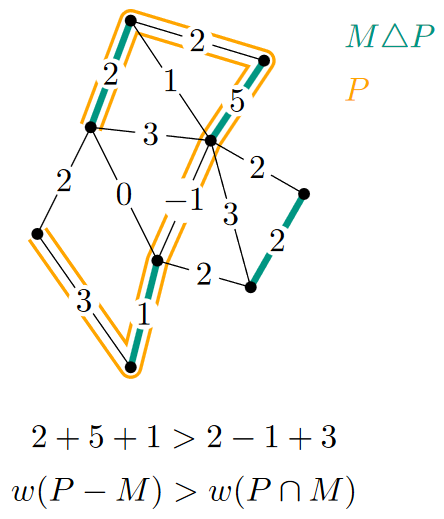
\includegraphics[width=0.25\textwidth]{images/sym-diff.png}
\end{center}
\bigskip
\textbf{Defintion}: Ein alternierender Weg heißt \textbf{erhöhend} wenn $w(M\Delta P)>w(M)$, also $w(P-M)>w(P\cap M)$.\\
\pagebreak

\textbf{Lemma}: Sei $M$ ein Matching in $(G, w)$. Es sind äquivalent:
\begin{itemize}
	\item $M$ ist gewichtsmaximal
	\item Es gibt keinen erhöhenden alternierenden Weg bezüglich $M$
\end{itemize}

\textit{Beweis}: 
\begin{itemize}
	\item \enquote{$\Rightarrow$}: Falls es zu $M$ einen erhöhenden Weg gibt, so kann $M$ natürlich nicht maximales Gewicht haben
	\item \enquote{$\Leftarrow$}: 
	\begin{itemize}
		\item Sei $M$ nicht gewichtsmaximal, also gibt es Matching $M^*$ mit $w(M^*)>w(M)$
		\item Betrachte $M\Delta M^*=(M\cup M^*)\setminus(M\cap M^*)$
		\begin{center}
			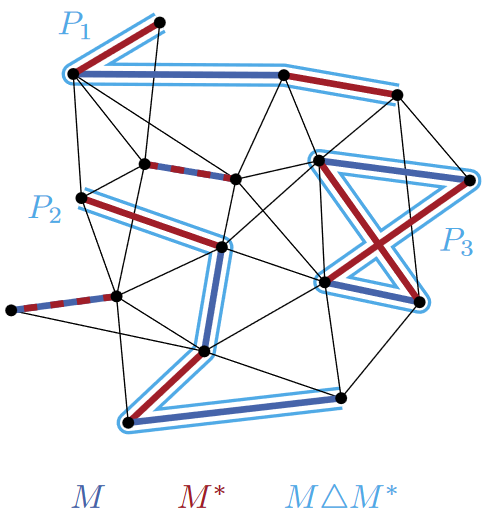
\includegraphics[width=0.25\textwidth]{images/moag1.png}
		\end{center}
		\item $M\Delta M^*$ hat nur Knoten vom Grad 1 oder 2, besteht also aus einfachen Kreisen und Wegen $P_1,\ldots, P_t$
		\item Jedes $P_i$ ist $M$-alternierender Weg
		\item Es gilt $w(M^*)-w(M)=\sum\limits_{i=1}^t (w(M^*-P_i)-w(M\cap P_i))$
		\item Ein Summand ist positiv, da $w(M^*)-w(M)>0$
		\item Einer der $P_i$ ist also erhöhend, mit $w(M^*\cap P_i)>w(P_i\cap M)$ $\implies$ Es gibt also einen erhöhenden Weg. Widerspruch.
	\end{itemize}
\end{itemize}
\bigskip
\textbf{Algorithmus für gewichtsmaximales Matching in planaren Graphen}: 
\begin{enumerate}
	\item Falls $|V(G)|\leq 5$, finde gewichtsmaximales Matching durch Brute-Force
	\item Falls $|V(G)|> 5$:
	\begin{itemize}
		\item Finde $\frac{2}{3}$-balancierten Separator $S$ mit $|S|=\mathcal{O}(\sqrt{n})$
		\item Berechne optimale Matchings auf allen Komponenten von $G'\coloneqq G-S$
		\item Sei $M'$ die Vereinigung dieser optimalen Matchings. $M'$ ist optimal für $G'$
	\end{itemize} 
	\pagebreak

	\item Solange $S\neq\emptyset$:
	\begin{itemize}
		\item Wähle $v\in S$. Finde alternierenden Weg $P$ in $G'+v$ mit Endpunkt $v$ mit $w(P-M')-w(P\cap M')$ maximal
		\item Falls $P$ erhöhend, ersetze $M'$ durch $M\Delta P$
		\item Lösche $v$ aus $S$
		\item Ersetze $G'$ durch $G'+v$
	\end{itemize}
\end{enumerate}

Im Folgenden wollen wir die Korrektheit des Algorithmus beweisen und dessen Laufzeit bestimmen. Mit folgendem Lemma folgt die Korrektheit.\\

\textbf{Lemma}: Sei $G=(V,E)$ ein Graph, $v\in V$ ein Knoten, $M$ ein gewichtsmaximales Matching in $G-v$. 
\begin{itemize}
	\item $M$ ist gewichtsmaximal in $G$ $\iff$ Es ex. kein erhöhender Weg mit Endpunkt $v$
\end{itemize}
Wenn ein erhöhender Pfad $P$ mit Endpunkt $v$ und $M'=M\Delta P$ existiert, dann gilt:
\begin{itemize}
	\item $M'$ ist gewichtsmaximal in $G$ $\iff$ Differenz $w(P-M)-w(P\cap M)$ ist maximal unter all solchen Pfaden mit Endpunkt $v$
\end{itemize}

\textit{Beweis - Teil 1}:
 \begin{itemize}
 	\item \enquote{$\Rightarrow$}: Wenn es einen solchen erhöhenden Weg gibt, dann kann $M$ nicht gewichtsmaximal in $G$ sein.
 	\item \enquote{$\Leftarrow$}:
 	\begin{itemize}
 		\item Sei $M$ nicht gewichtsmaximal in $G$, dann gibt es ein Matching $M^*$ mit $w(M^*)>w(M)$
 		\item Betrachte Pfade und Kreise $P_1,\ldots,P_t$ in $M\Delta M^*$
 		\item Analog zum letzten Beweis gibt es $P_i$ mit $w(M^*\cap P_i)>w(M\cap P_i)$
 		\item Wenn $v\notin P_i$, dann ist $P_i$ erhöhend für $M$ in $G-v$ $\implies$ Widerspruch, da angenommen wurde, dass $M$ optimales Matching für $G-v$ ist
 		\item Also ist $v\in P$. Da $v\notin M$, weil $M$ Matching für $G-v$ ist, ist $v$ ein Endpunkt von $P_i$
 	\end{itemize}
	 \begin{center}
	 	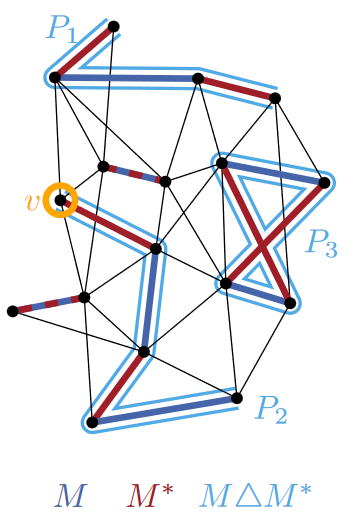
\includegraphics[width=0.17\textwidth]{images/moag2.png}
	 \end{center}
 \end{itemize}
\bigskip
\textit{Beweis - Teil 2}: 
\begin{itemize}
	\item \enquote{$\Rightarrow$}: Klar. Wenn $M'$ maximal ist, dann kann es keinen besseren Pfad geben.
	\item \enquote{$\Leftarrow$}: 
	\begin{itemize}
		\item Sei nicht $M'$, sondern $M^*$ gewichtsmaximal in $G$
		\item Analog zu oben gibt es erhöhenden Pfad $P$ in $M\Delta M^*$ mit $v$ als Endpunkt (da nur Komponente mit $v$ zu Verbesserung führen kann, weil andere Komponenten auch von $M$ betrachtet wurden) und $w(M^*)-w(M)=w(P-M)-w(P\cap M)$
		\item Da $w(M^*)-w(M)>w(M')-w(M)$ war Pfad für $M'$ nicht maximal
	\end{itemize}
\end{itemize}
\bigskip
\textbf{Satz}: Ein gewichtsmaximales Matching eines planaren Graphen mit $n$ Knoten kann in $\mathcal{O}(n^{\frac{3}{2}}\log n)$ berechnet werden.

\textit{Beweis}: Siehe Algorithmus für gewichtsmaximales Matching in planaren Graphen.
\begin{itemize}
	\item 1. geht in $\mathcal{O}(1)$
	\item Finden eines $\frac{2}{3}$-balancierten Separator in $\beta \cdot n$ Schritten
	\item Finden eines alternierenden Weges mit Endpunkt $v$ geht in $\mathcal{O}(n\cdot |S|)\leq \gamma\cdot n^{\frac{3}{2}}$ Schritten (s. Übung)
	\item Sei $T(n)$ die worst-case Gesamtlaufzeit, dann ist $T(n)\leq T(n_1)+T(n_2)+\beta\cdot n+\gamma\cdot n^{\frac{3}{2}}$, wobei $n_1,n_2$ die Anzahl der Knoten der Teilgraphen nach dem Separieren ist
	\item Der Rest vom Beweis ist viel Mathe und nicht relevant für die Klausur
\end{itemize}